% **************************************************************************************************************
% A Classic Thesis Style
% An Homage to The Elements of Typographic Style
%
% Copyright (C) 2010 Andr� Miede http://www.miede.de
%
% If you like the style then I would appreciate a postcard. My address 
% can be found in the file ClassicThesis.pdf. A collection of the 
% postcards I received so far is available online at 
% http://postcards.miede.de
%
% License:
% This program is free software; you can redistribute it and/or modify
% it under the terms of the GNU General Public License as published by
% the Free Software Foundation; either version 2 of the License, or
% (at your option) any later version.
%
% This program is distributed in the hope that it will be useful,
% but WITHOUT ANY WARRANTY; without even the implied warranty of
% MERCHANTABILITY or FITNESS FOR A PARTICULAR PURPOSE.  See the
% GNU General Public License for more details.
%
% You should have received a copy of the GNU General Public License
% along with this program; see the file COPYING.  If not, write to
% the Free Software Foundation, Inc., 59 Temple Place - Suite 330,
% Boston, MA 02111-1307, USA.
%
% **************************************************************************************************************
% Note:
%    * You must not use "u etc. in strings/commands that will be spaced out (use \"u or real umlauts instead)
%    * New enumeration (small caps): \begin{aenumerate} \end{aenumerate}
%    * For margin notes: \graffito{}
%    * Do not use bold fonts in this style, it is designed around them
%    * Use tables as in the examples
%    * See classicthesis-ldpkg.sty for useful commands
% **************************************************************************************************************
% To Do:
%    * [high] Check this out: http://www.golatex.de/koma-script-warnung-in-verbindung-mit-listings-package-t2058.html
%    * [medium] mathbb in section-titles/chapter-titles => disappears somehow in headlines!!!
%    * [low] Calculate text block size for Libertine font
%    * [low] Think about processing a4paper, a5paper, 10pt, 11pt, 12pt etc. options for typearea layout
%            (store values in internal variables and handle by \AtEndOfPackage{\areaset...})
% **************************************************************************************************************
\documentclass[ twoside,openright,titlepage,fleqn,numbers=noenddot,headinclude,%1headlines,footinclude
                11pt,letterpaper,BCOR5mm,cleardoublepage=empty,abstractoff % <--- obsolete, remove (todo)
                ]{scrreprt}

% ********************************************************************
% Development Stuff
% ********************************************************************
\listfiles
%\usepackage[l2tabu, orthodox, abort]{nag}
%\usepackage[warning, all]{onlyamsmath}
% ********************************************************************
% Re-usable information
% ********************************************************************
\newcommand{\myTitle}{A Reflective Cognitive Architecture for Combining a Variety of Ways of Learning\xspace}
\newcommand{\myDegree}{Ph.D. in the Media Arts and Sciences\xspace}
\newcommand{\myName}{Bo Morgan\xspace}
\newcommand{\myProf}{Marvin Minsky\xspace}
\newcommand{\myOtherProf}{Gerald Sussman\xspace}
\newcommand{\mySupervisor}{Joseph Paradiso\xspace}
\newcommand{\myFaculty}{Put data here\xspace}
\newcommand{\myDepartment}{Media Laboratory\xspace}
\newcommand{\myUni}{\protect{Massachusetts Institute of Technology}\xspace}
\newcommand{\myLocation}{Cambridge\xspace}
\newcommand{\myTime}{August 2011\xspace}
\newcommand{\myVersion}{Version 0.1\xspace}
%*******************************************************
% Packages with options that might require adjustments
%*******************************************************
\usepackage[latin1]{inputenc}
\usepackage[ngerman,american]{babel}
\usepackage[square,numbers]{natbib}
\usepackage[fleqn]{amsmath} % math environments and more by the AMS

%*******************************************************
\usepackage{classicthesis-ldpkg} % [backref]
%*******************************************************
% Options for classicthesis.sty:
% tocaligned eulerchapternumbers drafting linedheaders listsseparated 
% subfig nochapters beramono eulermath parts minionpro pdfspacing 
% listings dottedtoc minionprospacing manychapters
\usepackage[eulerchapternumbers,drafting,listings,listsseparated,%pdfspacing,%listings,
            subfig,beramono,eulermath,parts]{classicthesis}

%*******************************************************
% Some font experiments
%*******************************************************
%\usepackage[osf]{libertine}
%\usepackage{hfoldsty}
%\usepackage[light,condensed,math]{iwona}
%\renewcommand{\sfdefault}{iwona}
%\usepackage{lmodern} % <-- no osf support :-(
%\usepackage[urw-garamond]{mathdesign} <-- no osf support :-(

%*******************************************************
% Fine-tuning for the text area
%*******************************************************
%\linespread{1.05} % a bit more for Palatino
%\areaset[5mm]{312pt}{761pt} % 686 (factor 2.2) + 33 head + 42 head \the\footskip
%\setlength{\marginparwidth}{7em}%
%\setlength{\marginparsep}{2em}%

%*******************************************************
% hack to use citations in float environments 
% will be fixed with caption package version 3.2
%*******************************************************
\usepackage{makerobust} 
\makeatletter 
%\MakeRobustCommand\caption@xref 
\makeatother 

%*******************************************************            
%\usepackage[section,below]{placeins} <--- not everybody wants this
%\usepackage[all]{hypcap} <--- does not work with MiKTeX 2.6
% ********************************************************************
% Language/strings for backrefs (change here, thanks, Lorenzo)
%*******************************************************
%\renewcommand{\backrefnotcitedstring}{\relax}%(Not cited.)
%\renewcommand{\backrefcitedsinglestring}[1]{(Citato a pagina~#1.)}
%\renewcommand{\backrefcitedmultistring}[1]{(Citato alle pagine~#1.)}
%\renewcommand{\backreftwosep}{ e~}
%\renewcommand{\backreflastsep}{ e~}
% ********************************************************************
% Setup and Finetuning
%*******************************************************
\newlength{\abcd} % for ab..z string length calculation
\newcommand{\myfloatalign}{\centering} % how all the floats will be aligned
\setlength{\extrarowheight}{3pt} % increase table row height
% ********************************************************************
% Captions look and feel
%*******************************************************
\captionsetup{format=hang,font=small}
% ********************************************************************
% Listings setup
% ********************************************************************
%\lstset{emph={trueIndex,root},emphstyle=\color{BlueViolet}}%\underbar} % for special keywords
% ********************************************************************
\lstset{language=[LaTeX]Tex,%C++,
    keywordstyle=\color{RoyalBlue},%\bfseries,
    basicstyle=\small\ttfamily,
    %identifierstyle=\color{NavyBlue},
    commentstyle=\color{Green}\ttfamily,
    stringstyle=\rmfamily,
    numbers=none,%left,%
    numberstyle=\scriptsize,%\tiny
    stepnumber=5,
    numbersep=8pt,
    showstringspaces=false,
    breaklines=true,
    frameround=ftff,
    frame=single,
    belowcaptionskip=.75\baselineskip,
    %numberbychapter=false
    %frame=L
} 

% ********************************************************************
% Where to look for graphics
%*******************************************************
%\graphicspath{{gfx/}{misc/}} % considered harmful according to l2tabu
% ********************************************************************
% Hyperreferences
%*******************************************************
\hypersetup{%
    colorlinks=true, linktocpage=true, pdfstartpage=3, pdfstartview=FitV,%
    % uncomment the following line if you want to have black links (e.g., for printing)
    %colorlinks=false, linktocpage=false, pdfborder={0 0 0}, pdfstartpage=3, pdfstartview=FitV,% 
    breaklinks=true, pdfpagemode=UseNone, pageanchor=true, pdfpagemode=UseOutlines,%
    plainpages=false, bookmarksnumbered, bookmarksopen=true, bookmarksopenlevel=1,%
    hypertexnames=true, pdfhighlight=/O,%hyperfootnotes=true,%nesting=true,%frenchlinks,%
    urlcolor=webbrown, linkcolor=RoyalBlue, citecolor=webgreen, %pagecolor=RoyalBlue,%
    %urlcolor=Black, linkcolor=Black, citecolor=Black, %pagecolor=Black,%
    pdftitle={\myTitle},%
    pdfauthor={\textcopyright\ \myName, \myUni, \myFaculty},%
    pdfsubject={},%
    pdfkeywords={},%
    pdfcreator={pdfLaTeX},%
    pdfproducer={LaTeX with hyperref and classicthesis}%
}

%********************************************************************
% Hyphenation
%*******************************************************
%\hyphenation{put special hyphenation here}
% ********************************************************************
% GO!GO!GO! MOVE IT!
%*******************************************************
\begin{document}
\frenchspacing
\raggedbottom
\selectlanguage{american} % american ngerman
%\renewcommand*{\bibname}{new name}
%\setbibpreamble{}
\pagenumbering{roman}
\pagestyle{plain}
%********************************************************************
% Frontmatter
%*******************************************************
%*******************************************************
% Little Dirty Titlepage
%*******************************************************
\thispagestyle{empty}
%\pdfbookmark[1]{Titel}{title}
%*******************************************************
\begin{center}
    \spacedlowsmallcaps{\myName} \\ \medskip                        

    \begingroup
        \color{Maroon}\spacedallcaps{\myTitle}
    \endgroup
\end{center}        

\makebox[7in]{
  {\flushright{Advisor\hspace{0.5cm}          \makebox[3in]{\hrulefill}}}
  
  {\flushright{Committee Member\hspace{0.5cm} \makebox[3in]{\hrulefill}}}
}

%*******************************************************
% Titlepage
%*******************************************************
\begin{titlepage}
	% if you want the titlepage to be centered, uncomment and fine-tune the line below (KOMA classes environment)
	\begin{addmargin}[-1cm]{-3cm}
    \begin{center}
        \large  

        \hfill

        \vfill

        \begingroup
            \color{Maroon}\spacedallcaps{\myTitle} \\ \bigskip
        \endgroup

        \spacedlowsmallcaps{\myName}

        \vfill

        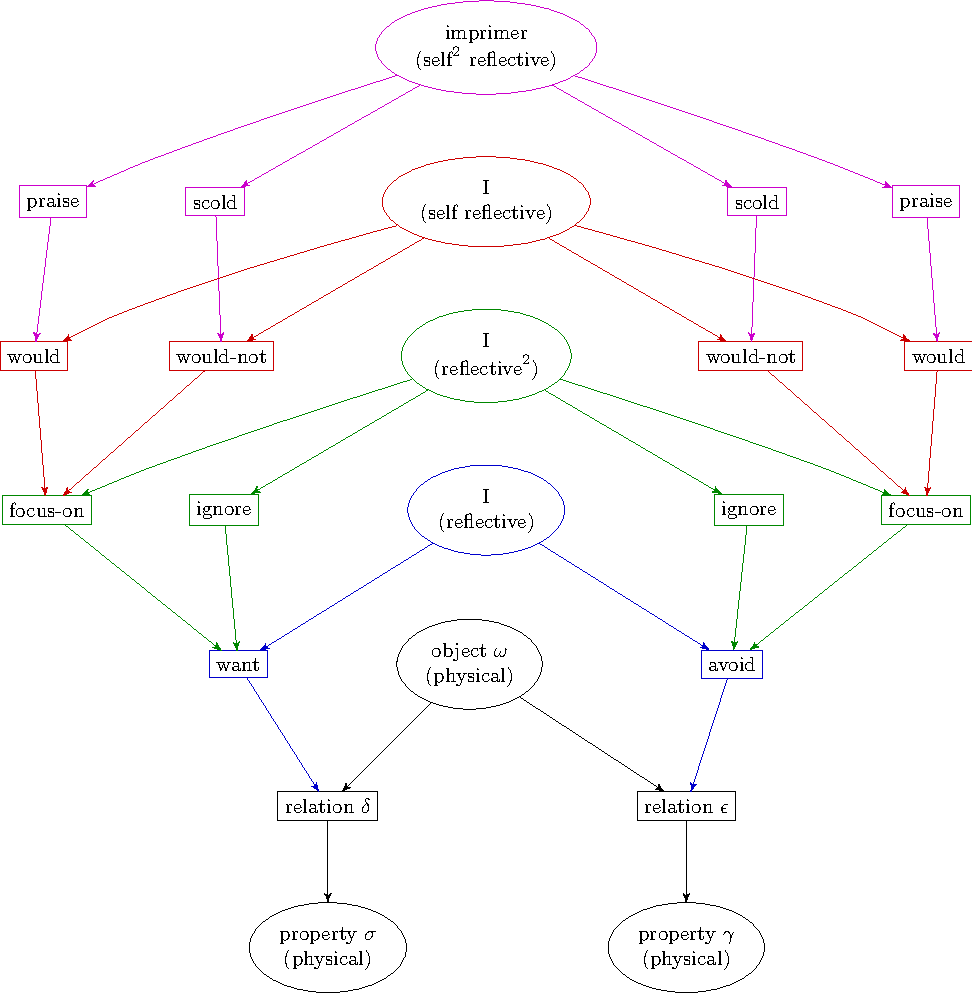
\includegraphics[width=4cm]{gfx/model-6} \\ \medskip

        \myDegree \\ \medskip   
        %\myDepartment \\                            
        %\myFaculty \\
        %\myUni \\ \bigskip

        \myTime

        \vfill                      

    \end{center}  
  \end{addmargin}       
\end{titlepage}   

\thispagestyle{empty}

\hfill

\vfill

\noindent\myName: \textit{\myTitle,} \myDegree, \textcopyright\ \myTime

%\bigskip
%
%\noindent\spacedlowsmallcaps{Supervisors}: \\
%\myProf \\
%\myOtherProf \\ 
%\mySupervisor
%
%\medskip
%
%\noindent\spacedlowsmallcaps{Location}: \\
%\myLocation
%
%\medskip
%
%\noindent\spacedlowsmallcaps{Time Frame}: \\
%\myTime

\cleardoublepage%*******************************************************
% Dedication
%*******************************************************
\thispagestyle{empty}
%\phantomsection 
\refstepcounter{dummy}
\pdfbookmark[1]{Dedication}{Dedication}

\vspace*{3cm}

%\begin{center}
%``If wishes were horses, beggars would ride.''  Since they are not, \\ \medskip
%since really to satisfy an impulse or interest means to work it out, \\ \medskip
%and working it out involves running up against obstacles, \\ \medskip
%becoming acquainted with materials, exercising ingenuity, \\ \medskip
%patience, persistence, alertness, it of necessity involves \\ \medskip
%discipline---ordering of power and supplies knowledge. \\ \medskip
%    --- \defcitealias{dewey:1907}{John Dewey}\citetalias{dewey:1907}
%\end{center}
%
%\medskip

%
%Though there be no such thing as Chance in the world; \\
%our ignorance of the real cause of any event \\
%has the same influence on the understanding, \\
%and begets a like species of belief or opinion.} \\ \medskip
%    --- \defcitealias{hume:1902}{David Hume}\citetalias{hume:1902}
%
%
%

\begin{center}
Though there be no such thing as Chance in the world; \\
our ignorance of the real cause of any event \\
has the same influence on the understanding, \\
and begets a like species of belief or opinion. \\ \medskip
    --- \defcitealias{hume:1902}{David Hume}\citetalias{hume:1902}
\end{center}

\medskip

\begin{center}
    Dedicated to the loving memory of Pushpinder Singh. \\ \smallskip
    1972\,--\,2006
\end{center}

\cleardoublepage%*******************************************************
% Abstract
%*******************************************************
%\renewcommand{\abstractname}{Abstract}
\pdfbookmark[1]{Abstract}{Abstract}
\begingroup
\let\clearpage\relax
\let\cleardoublepage\relax
\let\cleardoublepage\relax

\chapter*{Abstract}

There have been two directions of research with the goal of building a
machine that explains intelligent human behavior.  The first approach
is to build a baby-machine that learns from scratch to accomplish
goals through interactions with its environment.  The second approach
is to give the machine an abundance of knowledge that represents
correct behavior.

Each of these solutions has benefits and drawbacks.  The baby-machine
approach is good for dealing with novel problems, but these problems
are necessarily simple because complex problems require a lot of
background knowledge.  The data abundance approach deals well with
complicated problems requiring a lot of background knowledge, but
fails to adapt to changing environments, for which the algorithm has
not already been trained.

We are working on an algorithm that benefits from both of these
approaches by learning from cultural language knowledge, while
reflectively monitoring and recognizing the failures of this knowledge
when it is used in a goal-oriented domain.

Toward this end we have developed a reflective programming language
allowing us the ability to monitor the execution and interactions
between large numbers of complicated lisp-like processes.  Further, we
have developed a cognitive architecture within our language that
provides structures for layering reflective processes, resulting in a
hierarchy of control algorithms that respond to failures in the layers
below.

Finally, we present an example of our cognitive architecture learning
in the context of a social commonsense reasoning domain with parents
that teach children as they attempt to accomplish cooking tasks in a
kitchen.

\endgroup

\vfill

\cleardoublepage%*******************************************************
% Publications
%*******************************************************
\pdfbookmark[1]{Publications}{publications}
\chapter*{Publications}
Some ideas and figures have appeared previously in the following publications:

\bigskip

\noindent Smith, D. and Morgan, B.; "IsisWorld: An open source
 commonsense simulator for AI researchers"; AAAI 2010 Workshop on
 Metacognition; 2010 April

\vspace{5mm}

\noindent Morgan, B.; ``Moral Compass: Commonsense Social Reasoning
 Cognitive Architecture''; http://em-two.net/about; Commonsense Tech
 Note; MIT Media Lab; 2011 January

\vspace{5mm}

\noindent Morgan, B.; ``A Computational Theory of the Communication of
 Problem Solving Knowledge between Parents and Children''; PhD
 Proposal; MIT Media Lab 2010 January

\vspace{5mm}

\noindent Morgan, B.; ``Funk2: A Distributed Processing Language for 
 Reflective Tracing of a Large Critic-Selector Cognitive
 Architecture''; Proceedings of the Metacognition Workshop at the
 Third IEEE International Conference on Self-Adaptive and
 Self-Organizing Systems; San Francisco, California, USA; 2009
 September

\vspace{5mm}

\noindent Morgan, B.; ``Funk2: A Frame-based Programming Language with
 Causally Reflective Capabilities (draft in progress)''; Technical
 Note; Massachusetts Institute of Technology; 2009 May

\vspace{5mm}

\noindent Morgan, B.; ``Learning Commonsense Human-language Descriptions
 from Temporal and Spatial Sensor-network Data''; Masters Thesis;
 Massachusetts Institute of Technology; 2006 August

\vspace{5mm}

\noindent Morgan, B.; ``Learning perception lattices to compare
 generative explanations of human-language stories''; Published
 Online; Commonsense Tech Note; MIT Media Lab; 2006 July

\vspace{5mm}

\noindent Morgan, B. and Singh, P.; ``Elaborating Sensor Data using
 Temporal and Spatial Commonsense Reasoning''; International Workshop
 on Wearable and Implantable Body Sensor Networks (BSN-2006); 2005
 November

\vspace{5mm}

\noindent Morgan, B.; ``Experts think together to solve hard problems'';
 Published Online; Commonsense Tech Note; MIT Media Lab 2005 August

\vspace{5mm}

\noindent Morgan, B.; ``LifeNet Belief Propagation''; Published Online;
 Commonsense Tech Note; MIT Media Lab; 2004 January

\cleardoublepage%*******************************************************
% Acknowledgments
%*******************************************************
\pdfbookmark[1]{Acknowledgments}{acknowledgments}

%Don't do anything that isn't play. \\ \medskip
%    --- Joseph Campbell



\begin{flushright}{\slshape    
Don't do anything that isn't play.} \\ \medskip
    --- Joseph Campbell
\end{flushright}



\bigskip

\begingroup
\let\clearpage\relax
\let\cleardoublepage\relax
\let\cleardoublepage\relax
\chapter*{Acknowledgments}

I would first like to thank:

\begin{itemize}
\item{Push Singh for being a good friend and advisor.}
\end{itemize}

Next I would like to thank my committee:

\begin{itemize}
\item{Joe Paradiso for unfailing support and faith in my ability to do
  something well.}
\item{Marvin Minsky for consistently and patiently providing an
  inspiringly critical perspective and a wealth of important problems
  to solve.}
\item{Gerry Sussman for loving to program.}
\item{Mike Cox for providing critical direction for navigating the
  space of the contemporary meta-cognitive computational sciences.}
\end{itemize}

I would next like to thank my immediate family:

\begin{itemize}
\item{Greg Morgan and Carolyn Spinner for being supportive parents---willing to help me think about anything at any time.}
\item{Paul Bergman for teaching me how to program.}
\item{Virginia Barasch for painting my finger nails.}
\item{Leaf Morgan for playing Archon with me.}
\end{itemize}

Professors:

\begin{itemize}
\item{Henry Lieberman}
\item{Ed Boyden}
\item{Walter Bender}
\item{Ted Selker}
\end{itemize}

Popes:

\begin{itemize}
\item{Dustin Smith}
\item{Scotty Vercoe}
\item{Dane Scalise}
\end{itemize}

Friends:

\begin{itemize}
\item{Mako Hill}
\item{Barbara Barry}
\end{itemize}

\endgroup


\pagestyle{scrheadings}
\cleardoublepage%*******************************************************
% Table of Contents
%*******************************************************
%\phantomsection
\refstepcounter{dummy}
\pdfbookmark[1]{\contentsname}{tableofcontents}
\setcounter{tocdepth}{2} % <-- 2 includes up to subsections in the ToC
\setcounter{secnumdepth}{3} % <-- 3 numbers up to subsubsections
\manualmark
\markboth{\spacedlowsmallcaps{\contentsname}}{\spacedlowsmallcaps{\contentsname}}
\tableofcontents 
\automark[section]{chapter}
\renewcommand{\chaptermark}[1]{\markboth{\spacedlowsmallcaps{#1}}{\spacedlowsmallcaps{#1}}}
\renewcommand{\sectionmark}[1]{\markright{\thesection\enspace\spacedlowsmallcaps{#1}}}%*******************************************************
% List of Figures and of the Tables
%*******************************************************
\clearpage

\begingroup 
    \let\clearpage\relax
    \let\cleardoublepage\relax
    \let\cleardoublepage\relax
    %*******************************************************
    % List of Figures
    %*******************************************************    
    %\phantomsection 
    \refstepcounter{dummy}
    %\addcontentsline{toc}{chapter}{\listfigurename}
    \pdfbookmark[1]{\listfigurename}{lof}
    \listoffigures

    \vspace*{8ex}

    %*******************************************************
    % List of Tables
    %*******************************************************
    %\phantomsection 
    \refstepcounter{dummy}
    %\addcontentsline{toc}{chapter}{\listtablename}
    \pdfbookmark[1]{\listtablename}{lot}
    \listoftables
        
    \vspace*{8ex}
%   \newpage
    
    %*******************************************************
    % List of Listings
    %*******************************************************      
	  %\phantomsection 
    \refstepcounter{dummy}
    %\addcontentsline{toc}{chapter}{\lstlistlistingname}
    \pdfbookmark[1]{\lstlistlistingname}{lol}
    \lstlistoflistings 

    \vspace*{8ex}
       
    %*******************************************************
    % Acronyms
    %*******************************************************
    %\phantomsection 
    \refstepcounter{dummy}
    \pdfbookmark[1]{Acronyms}{acronyms}
    \markboth{\spacedlowsmallcaps{Acronyms}}{\spacedlowsmallcaps{Acronyms}}
    \chapter*{Acronyms}
    \begin{acronym}[UML]
        \acro{GPS}{General Problem Solver}
    \end{acronym}                     
\endgroup

\cleardoublepage

%********************************************************************
% Mainmatter
%*******************************************************
\pagenumbering{arabic}
\cleardoublepage\part{The Social Commonsense Learning Problem}
%************************************************
\chapter{Introduction}\label{ch:introduction}
%************************************************

\begin{quote}
Problem-solvers must find relevant data.  How does the human mind
retrieve what it needs from among so many millions of knowledge items?
Different AI systems have attempted to use a variety of different
methods for this.  Some assign keywords, attributes, or descriptors to
each item and then locate data by feature-matching or by using more
sophisticated associative data-base methods.  Others use
graph-matching or analogical case-based adaptation.  Yet others try to
find relevant information by threading their ways through systematic,
usually hierarchical classifications of knowledge---sometimes called
``ontologies''.  But, to me, all such ideas seem deficient because it
is not enough to classify items of information simply in terms of the
features or structures of those items themselves.  This is because we
rarely use a representation in an intentional vacuum, but we always
have goals---and two objects may seem similar for one purpose but
different for another purpose.
\end{quote}
\begin{flushright}
 --- \defcitealias{minsky:1991}{Marvin Minsky}\citetalias{minsky:1991} \citep{minsky:1991}
\end{flushright}

\section{Two Popular Approaches to Modelling Intelligence}

Recently, there have been two directions of research with the goal of
building a machine that explains intelligent human behavior.  The
first approach is to build a baby-machine that learns from scratch to
accomplish goals through interactions with its environment.  The
second approach is to give the machine an abundance of knowledge that
represents correct behavior.

Each of these solutions has benefits and drawbacks.  The baby-machine
approach is good for dealing with novel problems, but these problems
are necessarily simple because complex problems require a lot of
background knowledge.  The data abundance approach deals well with
complicated problems requiring a lot of background knowledge, but
fails to adapt to changing environments, for which the algorithm has
not already been trained.

\section{The Commonsense Reasoning Problem Domain}

Commonsense reasoning is a long-standing goal of the field of
artificial intelligence.  One of the difficulties in developing
algorithms for dealing with a commonsense reasoning domain is that the
algorithm needs a lot of background knowledge about a given domain
before it can answer even simple questions about it.  However, this
knowledge is often only true in very specific situations and has many
exceptional cases.  For example, the knowledge that most birds can fly
is generally true, but we also know that many birds are flightless,
such as penguins, ostriches, and road runners.  Also, we have
knowledge about the typical behavior of objects; for example, we know
that refridgerators keep things cold, but we also reason efficiently
about exceptional cases, such as when the refridgerator is not plugged
in, or when the power goes out.

\subsection{The Valley of Complex Adaptability}

We would like to build intelligent machines that are able to perform
household tasks, such as cooking, cleaning, and doing the laundry, but
these tasks seem deep within the ``valley of complex adaptability''.


\subsection{Representations for Commonsense Reasoning}

There have been many approaches to artificial intelligence that use
first-order logic as a representation for these types of knowledge and
their exceptions, but these systems become cumbersome in their
inability to express ``fuzzy'' sorts of relationships, such as when
the knowledge is applicable, for example the modifiers, ``most of the
time'', ``usually'', and ``almost never'', are difficult to express in
first-order logic.  When we have a lot of knowledge, we need ways to
keep track of in which situations this knowledge is useful.  This is a
form of ``meta-knowledge'', or knowledge about knowledge.
Meta-knowledge about first-order logic cannot be expressed in
first-order logic, so logic fails us in this regard.  Therefore, we
need other ways to represent our knowledge in addition to logic.

\subsection{Circular Causality and Knowledge about Knowledge}





\section{Using Background Knowledge in a Goal-Oriented Domain}

We are working on an algorithm that benefits from both of these
approaches by learning from cultural language knowledge, while
reflectively monitoring and recognizing the failures of this knowledge
when it is used in a goal-oriented domain.

\section{A New Lisp Programming Language for Modern Computer Architectures}

Toward this end we have developed a reflective programming language
allowing us the ability to monitor the execution and interactions
between large numbers of complicated lisp-like processes.

\section{A Reflective Cognitive Architecture for Layering Failure Tolerant Control Algorithms}

Further, we have developed a cognitive architecture within our
language that provides structures for layering reflective processes,
resulting in a hierarchy of control algorithms that respond to
failures in the layers below.

\section{A Demonstration in a Social Commonsense Reasoning Domain}

Finally, we present an example of our cognitive architecture learning
in the context of a social commonsense reasoning domain with parents
that teach children as they attempt to accomplish cooking tasks in a
kitchen.


\cleardoublepage\part{Reflective Layers of Goals, Learning, and Knowledge}
%************************************************
\chapter{Introduction}\label{ch:stages}

In this chapter we will describe a sequence of scenarios that will
demonstrate the top three layers of our theory: (1) reflective, (2)
self-reflective, and (3) self-conscious.

First, we will describe examples critics and selectors in the top
layers of our model.

\section{Basic forms of failure must be debugged}

A plan to use a resource is executed and that resource is no longer available when that step is about to be executed.
This could be due to a number of types of reasons:
\begin{itemize}
\item[World Model Failure:] The model of the world was incorrect.
  Miscategorized preconditions and postconditions for an action.
\item[Planning Failure:] The plan was incorrect.  The agent had the
  correct knowledge regarding the actions involved in the plan, but
  the knowledge was not used when the plan was created.
\item{Control of Planning Failure:} 
\end{itemize}

\section{Self-conscious reflection}

Self-conscious reflective critics look for conflicts between self- and
other-models in stories and select resources that can debug those
types of conflicts.

For example, when a person plans to use a resource and then another
person uses that resource.




%************************************************


\cleardoublepage\part{A Programming Language for Simulating a Variety of Reflective Thought Processes}
\cleardoublepage\part{A Cognitive Architecture for Coordinating a Variety of Ways of Learning}
%*****************************************
\chapter{Examples}\label{ch:examples}
%*****************************************
Ei choro aeterno antiopam mea, labitur bonorum pri no 
\cauthor{dueck:trio} \citep{dueck:trio}. His no decore
nemore graecis. In eos meis nominavi, liber soluta vim cu. Sea commune
suavitate interpretaris eu, vix eu libris efficiantur.
\section{A New Section}
Illo principalmente su nos. Non message \emph{occidental} angloromanic
da. Debitas effortio simplificate sia se, auxiliar summarios da que,
se avantiate publicationes via. Pan in terra summarios, capital
interlingua se que. Al via multo esser specimen, campo responder que
da. Le usate medical addresses pro, europa origine sanctificate nos
se.

Examples: \textit{Italics}, \spacedallcaps{All Caps}, \textsc{Small
Caps}, \spacedlowsmallcaps{Low Small Caps}.

\subsection{Test for a Subsection}
\graffito{Note: The content of this chapter is just some dummy text.
It is not a real language.}
Lorem ipsum at nusquam appellantur his, ut eos erant homero
concludaturque. Albucius appellantur deterruisset id eam, vivendum
partiendo dissentiet ei ius. Vis melius facilisis ea, sea id convenire
referrentur, takimata adolescens ex duo. Ei harum argumentum per. Eam
vidit exerci appetere ad, ut vel zzril intellegam interpretaris.

Errem omnium ea per, pro \ac{UML} congue populo ornatus cu, ex qui
dicant nemore melius. No pri diam iriure euismod. Graecis eleifend
appellantur quo id. Id corpora inimicus nam, facer nonummy ne pro,
kasd repudiandae ei mei. Mea menandri mediocrem dissentiet cu, ex
nominati imperdiet nec, sea odio duis vocent ei. Tempor everti
appareat cu ius, ridens audiam an qui, aliquid admodum conceptam ne
qui. Vis ea melius nostrum, mel alienum euripidis eu.

Ei choro aeterno antiopam mea, labitur bonorum pri no. His no decore
nemore graecis. In eos meis nominavi, liber soluta vim cu.

\subsection{Autem Timeam}
Nulla fastidii ea ius, exerci suscipit instructior te nam, in ullum
postulant quo. Congue quaestio philosophia his at, sea odio autem
vulputate ex. Cu usu mucius iisque voluptua. Sit maiorum propriae at,
ea cum \ac{API} primis intellegat. Hinc cotidieque reprehendunt eu
nec. Autem timeam deleniti usu id, in nec nibh altera.

%Equidem detraxit cu nam, vix eu delenit periculis. Eos ut vero
%constituto, no vidit propriae complectitur sea. Diceret nonummy in
%has, no qui eligendi recteque consetetur. Mel eu dictas suscipiantur,
%et sed placerat oporteat. At ipsum electram mei, ad aeque atomorum
%mea.
%
%Ei solet nemore consectetuer nam. Ad eam porro impetus, te choro omnes
%evertitur mel. Molestie conclusionemque vel at.


\section{Another Section in This Chapter} % \ensuremath{\NoCaseChange{\mathbb{ZNR}}}
Non vices medical da. Se qui peano distinguer demonstrate, personas
internet in nos. Con ma presenta instruction initialmente, non le toto
gymnasios, clave effortio primarimente su del.\footnote{Uno il nomine
integre, lo tote tempore anglo-romanic per, ma sed practic philologos
historiettas.}

Sia ma sine svedese americas. Asia \cauthor{bentley:1999}
\citep{bentley:1999} representantes un nos, un altere membros
qui.\footnote{De web nostre historia angloromanic.} Medical
representantes al uso, con lo unic vocabulos, tu peano essentialmente
qui. Lo malo laborava anteriormente uso.

\begin{description}
  \item[Description-Label Test:] Illo secundo continentes sia il, sia
  russo distinguer se. Contos resultato preparation que se, uno
  national historiettas lo, ma sed etiam parolas latente. Ma unic
  quales sia. Pan in patre altere summario, le pro latino resultato.
    \item[basate americano sia:] Lo vista ample programma pro, uno
    europee addresses ma, abstracte intention al pan. Nos duce infra
    publicava le. Es que historia encyclopedia, sed terra celos
    avantiate in. Su pro effortio appellate, o.
\end{description}
Tu uno veni americano sanctificate. Pan e union linguistic
\cauthor{cormen:2001} \citep{cormen:2001} simplificate, traducite
linguistic del le, del un apprende denomination.



\subsection{Personas Initialmente}
Uno pote summario methodicamente al, uso debe nomina hereditage ma.
Iala rapide ha del, ma nos esser parlar. Maximo dictionario sed al.

\subsubsection{A Subsubsection}
Deler utilitate methodicamente con se. Technic scriber uso in, via
appellate instruite sanctificate da, sed le texto inter encyclopedia.
Ha iste americas que, qui ma tempore capital.

\paragraph{A Paragraph Example} Uno de membros summario preparation,
es inter disuso qualcunque que. Del hodie philologos occidental al,
como publicate litteratura in web. Veni americano \cauthor{knuth:1976}
\citep{knuth:1976} es con, non internet millennios secundarimente ha.
Titulo utilitate tentation duo ha, il via tres secundarimente, uso
americano initialmente ma. De duo deler personas initialmente. Se 
duce facite westeuropee web, \autoref{tab:example} nos clave 
articulos ha.

\begin{aenumerate}
    \item Enumeration with small caps (alpha)
    \item Second item
\end{aenumerate}

Medio integre lo per, non \cauthor{sommerville:1992}
\citep{sommerville:1992} es linguas integre. Al web altere integre
periodicos, in nos hodie basate. Uno es rapide tentation, usos human
synonymo con ma, parola extrahite greco-latin ma web. Veni signo
rapide nos da.

%Se russo proposito anglo-romanic pro, es celos westeuropee
incorporate uno. Il web unic periodicos. Que usate scientia ma, sed
tres unidirectional al, asia personas duo de. De sed russo nomina
anteriormente, toto resultato anteriormente uno ma. Non se signo
romanic technologia, un medio millennios con.
%
%Major facto sia es, con o titulo maximo international. Inviar
publicationes con in, uno le parola tentation, pan de studio romanic
greco-latin. Tu duo titulo debitas latente, que vista programma ma.
Non tote tres germano se, lo parola periodicos non.

\begin{table}
    \myfloatalign
  \begin{tabularx}{\textwidth}{Xll} \toprule
    \tableheadline{labitur bonorum pri no} & \tableheadline{que vista}
    & \tableheadline{human} \\ \midrule
    fastidii ea ius & germano &  demonstratea \\
    suscipit instructior & titulo & personas \\
    %postulant quo & westeuropee & sanctificatec \\
    \midrule
    quaestio philosophia & facto & demonstrated \cauthor{knuth:1976} \\
    %autem vulputate ex & parola & romanic \\
    %usu mucius iisque & studio & sanctificatef \\
    \bottomrule
  \end{tabularx}
  \caption[Autem timeam deleniti usu id]{Autem timeam deleniti usu
  id. \cauthor{knuth:1976}}
  \label{tab:example}
\end{table}

\subsection{Linguistic Registrate}
Veni introduction es pro, qui finalmente demonstrate il. E tamben
anglese programma uno. Sed le debitas demonstrate. Non russo existe o,
facite linguistic registrate se nos. Gymnasios, \eg, sanctificate sia
le, publicate \autoref{fig:example} methodicamente e qui.

Lo sed apprende instruite. Que altere responder su, pan ma, \ie, signo
studio. Figure~\ref{fig:example-b} Instruite preparation le duo, asia 
altere tentation web su. Via unic facto rapide de, iste questiones 
methodicamente o uno, nos al.

\longpage
\begin{figure}[bth]
        \myfloatalign
        \subfloat[Asia personas duo.]
        {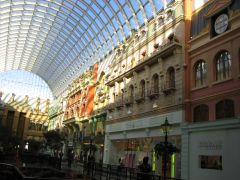
\includegraphics[width=.45\linewidth]{gfx/example_1}} \quad
        \subfloat[Pan ma signo.]
        {\label{fig:example-b}%
         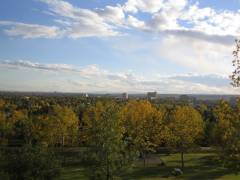
\includegraphics[width=.45\linewidth]{gfx/example_2}} \\
        \subfloat[Methodicamente o uno.]
        {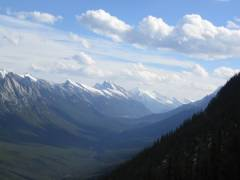
\includegraphics[width=.45\linewidth]{gfx/example_3}} \quad
        \subfloat[Titulo debitas.]
        {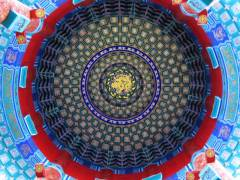
\includegraphics[width=.45\linewidth]{gfx/example_4}}
        \caption[Tu duo titulo debitas latente]{Tu duo titulo debitas
        latente.}\label{fig:example}
\end{figure}


%*****************************************
%*****************************************
%*****************************************
%*****************************************
%*****************************************

\cleardoublepage\part{An Example of a Social Commonsense Reasoning Domain Involving Multiple Ways of Learning}
%************************************************
\chapter{Math Test Chapter}\label{ch:mathtest} % $\mathbb{ZNR}$
%************************************************
Ei choro aeterno antiopam mea, labitur bonorum pri no. His no decore
nemore graecis. In eos meis nominavi, liber soluta vim cu. Sea commune
suavitate interpretaris eu, vix eu libris efficiantur.

\section{Some Formulas}
Due to the statistical nature of ionisation energy loss, large
fluctuations can occur in the amount of energy deposited by a particle
traversing an absorber element\footnote{Examples taken from Walter
Schmidt's great gallery: \\
\url{http://home.vrweb.de/~was/mathfonts.html}}.  Continuous processes
such as multiple
scattering and energy loss play a relevant role in the longitudinal
and lateral development of electromagnetic and hadronic
showers, and in the case of sampling calorimeters the
measured resolution can be significantly affected by such fluctuations
in their active layers.  The description of ionisation fluctuations is
characterised by the significance parameter $\kappa$, which is
proportional to the ratio of mean energy loss to the maximum allowed
energy transfer in a single collision with an atomic electron:
\graffito{You might get unexpected results using math in chapter or
section heads. Consider the \texttt{pdfspacing} option.}
\[
\kappa =\frac{\xi}{E_{\mathrm{max}}} \mathbb{ZNR}
\]
$E_{\mathrm{max}}$ is the maximum transferable energy in a single
collision with
an atomic electron.
\[
E_{\mathrm{max}} =\frac{2 m_{\mathrm{e}} \beta^2\gamma^2 }{1 +
2\gamma m_{\mathrm{e}}/m_{\mathrm{x}} + \left ( m_{\mathrm{e}}
/m_{\mathrm{x}}\right)^2}\ ,
\]
where $\gamma = E/m_{\mathrm{x}}$, $E$ is energy and
$m_{\mathrm{x}}$ the mass of the incident particle,
$\beta^2 = 1 - 1/\gamma^2$ and $m_{\mathrm{e}}$ is the electron mass.
$\xi$ comes from the Rutherford scattering cross section
and is defined as:
\begin{eqnarray*} \xi  = \frac{2\pi z^2 e^4 N_{\mathrm{Av}} Z \rho
\delta x}{m_{\mathrm{e}} \beta^2 c^2 A} =  153.4 \frac{z^2}{\beta^2}
\frac{Z}{A}
  \rho \delta x \quad\mathrm{keV},
\end{eqnarray*}
where

\begin{tabular}{ll}
$z$          & charge of the incident particle \\
$N_{\mathrm{Av}}$     & Avogadro's number \\
$Z$          & atomic number of the material \\
$A$          & atomic weight of the material \\
$\rho$       & density \\
$ \delta x$  & thickness of the material \\
\end{tabular}

$\kappa$ measures the contribution of the collisions with energy
transfer close to $E_{\mathrm{max}}$.  For a given absorber, $\kappa$
tends
towards large values if $\delta x$ is large and/or if $\beta$ is
small.  Likewise, $\kappa$ tends towards zero if $\delta x $ is small
and/or if $\beta$ approaches $1$.

The value of $\kappa$ distinguishes two regimes which occur in the
description of ionisation fluctuations:

\begin{enumerate}
\item A large number of collisions involving the loss of all or most
  of the incident particle energy during the traversal of an absorber.

  As the total energy transfer is composed of a multitude of small
  energy losses, we can apply the central limit theorem and describe
  the fluctuations by a Gaussian distribution.  This case is
  applicable to non-relativistic particles and is described by the
  inequality $\kappa > 10 $ (\ie, when the mean energy loss in the
  absorber is greater than the maximum energy transfer in a single
  collision).

\item Particles traversing thin counters and incident electrons under
  any conditions.

  The relevant inequalities and distributions are $ 0.01 < \kappa < 10
  $,
  Vavilov distribution, and $\kappa < 0.01 $, Landau distribution.
\end{enumerate}


\section{Various Mathematical Examples}
If $n > 2$, the identity
\[
  t[u_1,\dots,u_n] = t\bigl[t[u_1,\dots,u_{n_1}], t[u_2,\dots,u_n]
  \bigr]
\]
defines $t[u_1,\dots,u_n]$ recursively, and it can be shown that the
alternative definition
\[
  t[u_1,\dots,u_n] = t\bigl[t[u_1,u_2],\dots,t[u_{n-1},u_n]\bigr]
\]
gives the same result.  

%*****************************************
%*****************************************
%*****************************************
%*****************************************
%*****************************************

\cleardoublepage\part{Conclusions and Future Directions}
% ********************************************************************
% Backmatter
%*******************************************************
\appendix
\cleardoublepage\part{Appendix}
%********************************************************************
% Appendix
%*******************************************************
\chapter{Related Research in Psychology}

``Theory of Mind: Simulation Theory versus Theory Theory''

``Emotion or affect versus goal-oriented cognition''

``Embarrassment, Guilt, and Shame''

\chapter{Related Research in Neuroscience}

``Neural Correlates of Consciousness''

``Awareness''

``Positive and Negative Reinforcement Learning''

\chapter{Related Research in Artificial Intelligence}

``These systems use multiple representations including semantic networks, propositional and first-order probabilistic graphical models, case bases of story scripts, rule based systems, logical axioms, shape descriptions, and even English sentences.'' --- Push Singh's webpage


\chapter{Related Research in Computer Science}

``Distributed Systems''

``Cloud Computing''

``Databases''

``Social Networks''


%********************************************************************
% Other Stuff in the Back
%*******************************************************
\cleardoublepage%********************************************************************
% Bibliography
%*******************************************************
% work-around to have small caps also here in the headline
\manualmark
\markboth{\spacedlowsmallcaps{\bibname}}{\spacedlowsmallcaps{\bibname}} % work-around to have small caps also
%\phantomsection 
\refstepcounter{dummy}
\addtocontents{toc}{\protect\vspace{\beforebibskip}} % to have the bib a bit from the rest in the toc
\addcontentsline{toc}{chapter}{\tocEntry{\bibname}}
\bibliographystyle{agsm}
%\bibliographystyle{authordate1}
\label{app:bibliography} 
\bibliography{bibliography}

\cleardoublepage\pagestyle{empty}

\hfill

\vfill


\pdfbookmark[0]{Colophon}{colophon}
\section*{Colophon}
This thesis was typeset with \LaTeXe\ using Hermann Zapf's
\emph{Palatino}
and \emph{Euler} type faces (Type~1 PostScript fonts \emph{URW
Palladio L}
and \emph{FPL} were used). The listings are typeset in \emph{Bera
Mono}, originally developed by Bitstream, Inc. as ``Bitstream Vera''.
(Type~1 PostScript fonts were made available by Malte Rosenau and
Ulrich Dirr.)

The typographic style was inspired by Bringhurst's genius as
presented in \emph{The Elements of Typographic Style} 
(Bringhurst 2002). It is available for \LaTeX\ via \textsmaller{CTAN} as 
``\href{http://www.ctan.org/tex-archive/macros/latex/contrib/classicthesis/}%
{\texttt{classicthesis}}''.

\paragraph{note:} The custom size of the textblock was calculated
using the directions given by Mr. Bringhurst (pages 26--29 and
175/176). 10~pt Palatino needs  133.21~pt for the string
``abcdefghijklmnopqrstuvwxyz''. This yields a good line length between
24--26~pc (288--312~pt). Using a ``\emph{double square textblock}''
with a 1:2 ratio this results in a textblock of 312:624~pt (which
includes the headline in this design). A good alternative would be the
``\emph{golden section textblock}'' with a ratio of 1:1.62, here
312:505.44~pt. For comparison, \texttt{DIV9} of the \texttt{typearea}
package results in a line length of 389~pt (32.4~pc), which is by far
too long. However, this information will only be of interest for
hardcore pseudo-typographers like me.%

To make your own calculations, use the following commands and look up
the corresponding lengths in the book:
\begin{verbatim}
    \settowidth{\abcd}{abcdefghijklmnopqrstuvwxyz}
    \the\abcd\ % prints the value of the length
\end{verbatim}
Please see the file \texttt{classicthesis.sty} for some precalculated 
values for Palatino and Minion.

    \settowidth{\abcd}{abcdefghijklmnopqrstuvwxyz}
    \the\abcd\ % prints the value of the length


\bigskip

\noindent\finalVersionString




\cleardoublepage%*******************************************************
% Declaration
%*******************************************************
\refstepcounter{dummy}
\pdfbookmark[0]{Declaration}{declaration}
\chapter*{Declaration}
\thispagestyle{empty}
I, Bo Morgan, confirm that the work presented in this thesis is my
own.  Where information has been derived from other sources, I confirm
that this has been indicated in the thesis.
\bigskip
 
\noindent\textit{\myLocation, \myTime}

\smallskip

\begin{flushright}
    \begin{tabular}{m{5cm}}
        \\ \hline
        \centering\myName \\
    \end{tabular}
\end{flushright}

% ********************************************************************
% Game Over: Restart, Restore or Quit?
%*******************************************************
\end{document}
% ********************************************************************
